\chapter{系统设计}
\label{design}

本系统一共由三部分组成。为用户提供一个具有真实触感的增强现实引擎,需要通过LibISR和RGB-D摄像头结合起来进行物体识别和追踪,它们构成了后端引擎。同时,为了方便用户可以使用本系统进行编著和交互,前端基于Unity开发了一套应用程序用于编著实验,并且移植在Android移动端上,基于手机端实现了增强现实交互。为了将用户编著数据和后端物体追踪数据进行传输,使用了网络通信。

\begin{figure}[!htp]
  \centering
  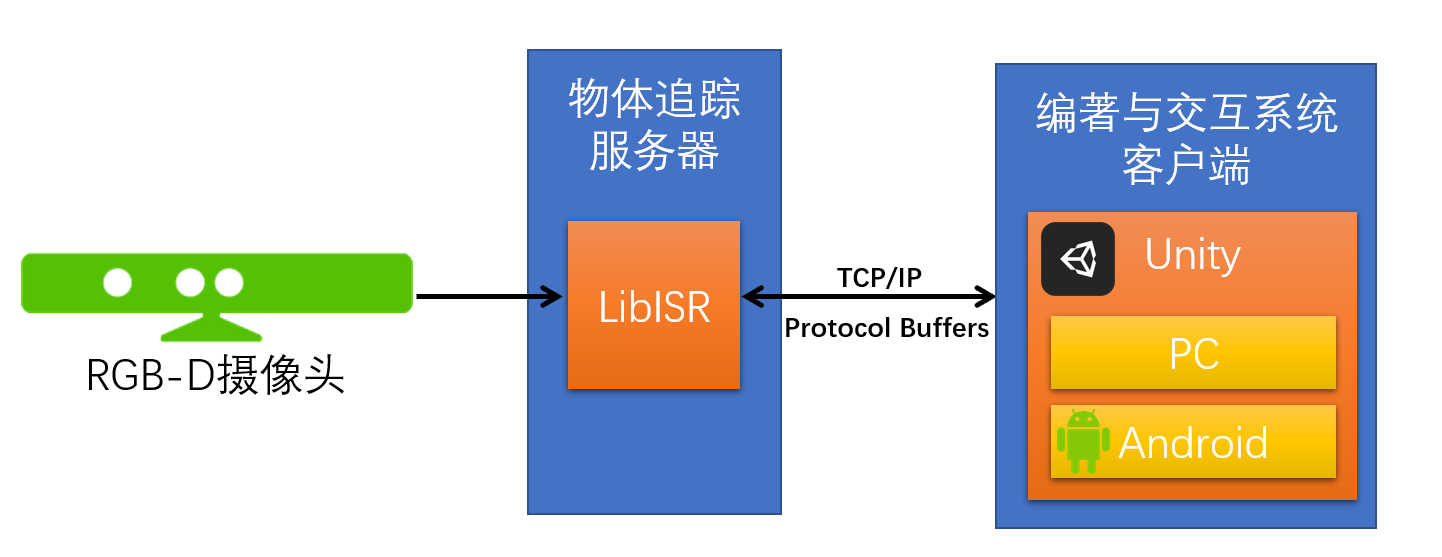
\includegraphics[width=12cm]{figure/TotalArc.png}
  \bicaption[系统架构图]
    {系统架构图}
    {The System Architecture Design}
 \label{fig:totalarc}
\end{figure}

综上所述,物体追踪引擎作为服务器,而编著和交互系统作为客户端,两者通过网络通信,本章节将会对这三部分的设计进行详细的介绍。

\section{服务器设计}

物体追踪引擎以LibISR为核心\cite{Ren_3DV_2014, star3d_iccv_2013},他的整体架构如图所示,其中只保留了比较核心以及在原程序上进行了一定修改的类。

\begin{figure}[!htp]
  \centering
  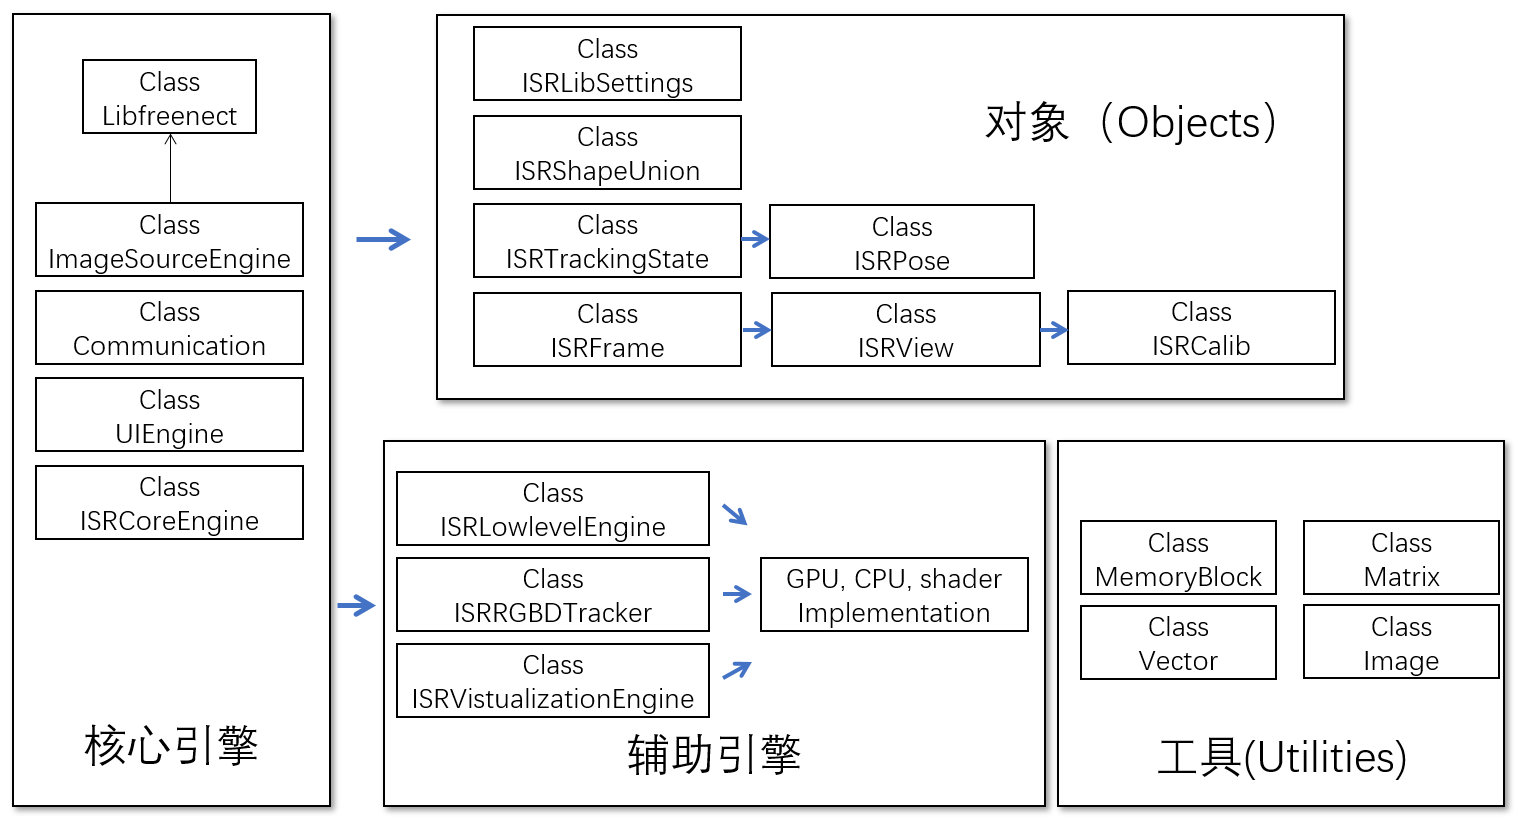
\includegraphics[width=12cm]{figure/LibArc.png}
  \bicaption[物体追踪架构图]
    {物体追踪架构图}
    {The Object Tracing Engine Architecture Design}
 \label{fig:labarc}
\end{figure}

LibISR是一个面向对象开发的应用,他的整体架构可以分为核心引擎、辅助引擎、对象、工具四部分。运行时,函数首先使用核心引擎进行初始化,包括使用的模型数据、追踪要求、标定数据等等,然后由负责网络通信、追踪计算、用户接口(UI)的引擎完成各自工作。这些工作涉及到的数据被封装为对象类。同时,LibISR还提供了一套自己的基础数据结构。

\subsection{对象}

对象是一些不包含业务逻辑,只负责将数据进行封装、整合、处理的类。首先对这些对象进行介绍,可以方便之后的讲述。

\begin{itemize}
    \item \textbf{ISRCalib}
用于储存标定数据,包括深度摄像头和彩色摄像头的内参、外参,以及单应性矩阵,这些标定数据又由单独的对象类进行储存。相机内外参数通过读取标定数据文件进行读取,而单质性矩阵则通过计算上述变量得出。
    
    \item \textbf{ISRPose}
储存物体的追踪结果,追踪结果由物体的旋转矩阵和位移向量组合起来的4x4矩阵。
    
    \item \textbf{ISRView}
储存相机读取的图像以及经过处理的中间数据。包括原始的彩色图像、深度图像,以及将彩色图对其到深度图之后的图像等。

    \item \textbf{ISRFrame}
储存了RGB-D图片的中间处理结果,例如点云、ISRView等。
    
    \item \textbf{ISRTracingState}
主要用于多物体追踪,保存所有物体的ISRPose,被用于计算代价函数。

    \item \textbf{ISRShapeUnion}
主要用于多物体追踪,保存由所有物体的模型组合而成的shape union。通过shape union可以讲多物体追踪和但物体追踪联系起来,提升了项目的可扩展性,但是本系统目前只是用了但物体追踪,因此不做详述。

    \item \textbf{ISRLibSettings}
保存项目的相关设置,包括是否使用GPU加速,是否追踪一种模型等。
\end{itemize}

\subsection{核心引擎}

核心引擎是暴露给用户的接口,负责启动物体追踪、获取摄像机数据、与网络传输数据、用户交互等核心功能。用户可以通过创建核心引擎的对象,从而实现物体追踪的功能。

\begin{itemize}
    \item \textbf{ImageSourceEngine}
该类是一个纯虚类,他负责连接硬件(摄像头),将读取到的数据进行数据格式转换、适配,保存在ISRView中,并将指针提供给其他引擎以供图片读取。
    
    \item \textbf{Communication}
该类用于传输网络数据,负责包括开启数据传输服务,等待前端用户输入并进行处理等功能。
    
    \item \textbf{UIEngine}
该类主要负责通过OpenGL Utility Toolkit(GLUT)实现用户前端,将追踪的原始RGB图像、深度图像、追踪结果、帧率等信息进行显示。并且通过glut的接口,循环调用图像处理函数,并且获得用户输入,包括开始、重置、暂停、录像等等。

    \item \textbf{ISRCoreEngine}
它是物体追踪的核心引擎。在每一帧都会运行,将获取的图片进行处理,调用ISRRGBDTracker对象进行计算,获得物体位置后更新ISRTrackingState等对象,并且调用ISRVisualisationEngine将追踪的结果使用OpenGL进行可视化,之后由UIEngine进行显示。

\end{itemize}

\subsection{辅助引擎}

辅助引擎是辅助ISRCoreEngine进行工作的类,包含部分业务逻辑。这三类都是纯虚类,会根据硬件情况采用C++代码或CUDA\cite{CUDARef}代码的实现。

\begin{itemize}
    \item \textbf{ISRLowlevelEngine}
该类负责融合RGBD图像、应用滤波、获得bounding box、根据RGBD图像获得点云数据等功能。
    
    \item \textbf{ISRRGBDTracker}
用于进行物体追踪的计算,包括标记像素的前后景类型、计算代价函数、计算Jacobian矩阵用于代价函数局部最小化等算法的实现。
    
    \item \textbf{ISRVisualisationEngine}
用于中间数据的可视化,以及最终结果的渲染,包括渲染被追踪的物体、渲染深度图、渲染SDF模型应用结果等。它会根据渲染的结果将半透明的物体渲染在图像中的对应位置上,之后与RGB-D图像进行叠加实现融合和可视化。

\end{itemize}

\subsection{工具}

LibISR基于C++基本的数据结构进行了进一步的封装,实现了向量(vector)、矩阵(matrix)、图像(image)、数据块(memory block)等数据结构。向量和矩阵在提供基本运算的基础上,还提供了针对于实际需求的成员变量名,例如Vector3具有r,g,b三个成员,或x,y,z三个成员。此外,图像数据还提供了保存为文件的函数。数据块则为了统一管理在CPU和GPU进行转换的数据而设计,系统中所有的图像都以这种形式存在,方便在CPU和GPU之间切换。

\section{编著与交互系统客户端设计}
前端基于Unity引擎进行实现。应用由Game Manager进行控制,包括应用当中的各个场景以及他们的切换逻辑。其中编著系统主要在Build Experiment场景中,而通过追踪技术与物体交互的部分则主要在Tracing Scene场景中,此外还设计了其他场景。本小节将对这些场景的设计进行介绍。

\begin{figure}[!htp]
  \centering
  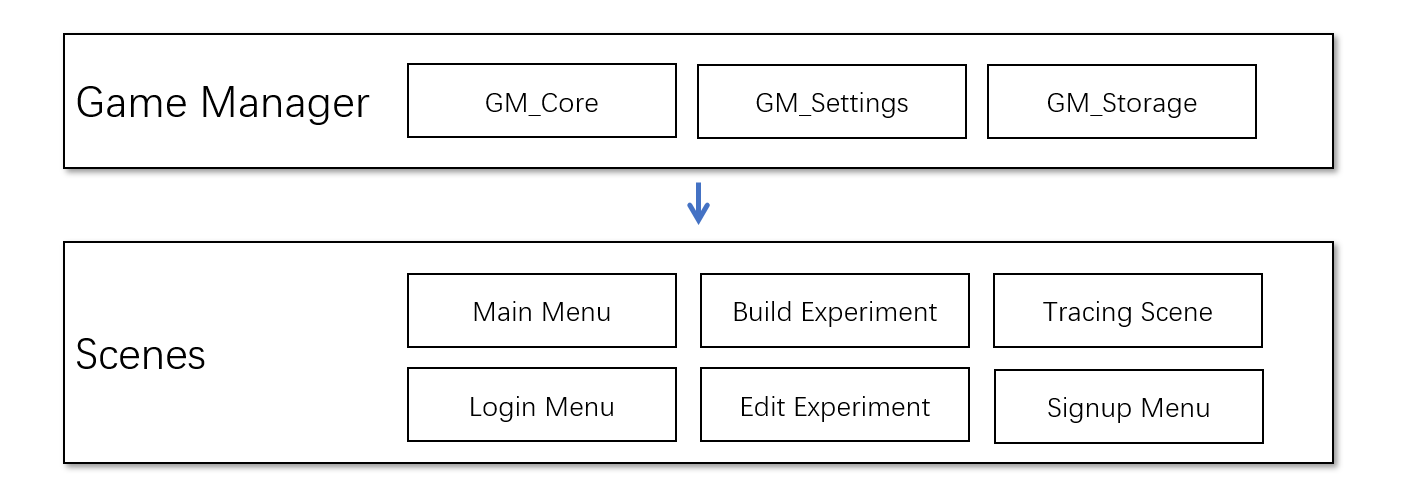
\includegraphics[width=12cm]{figure/GMarc.png}
  \bicaption[游戏管理器与场景架构设计图]
    {游戏管理器与场景架构设计图}
    {The Game Manager and Scenes Architecture Design}
 \label{fig:gm}
\end{figure}

\subsection{游戏管理器}
应用通过游戏管理器(Game Manager,GM)进行统一管理,负责的功能如下。
功能其一,它控制场景之间切换的异步加载逻辑并提供切换场景的接口,从而可以清晰、统一的管理所有场景之间的跳转逻辑。其二,它保存生命周期跨场景并且由用户产生的数据,保存这些数据的变量不能随着场景被切换而被销毁,也不可能在应用中以静态变量的形式存在,如登陆应用的账户信息、实验编著的结果等。其三,它提供了场景中静态变量的读取接口,因为这些变量需要在多个对象中使用,而且会随着应用开发进程产生变动,因此需要统一管理,包括系统支持的事件行为(化学操作如点燃酒精灯、连接导管等等)、器具类型、物质等等。而这些物体的信息则是保存在GM\_Storage中的。最后,由于在一部场景加载的时候,场景的光照设置是不会被修改的,因此不同于其他场景的光照,例如天空盒,需要针对每个场景进行单独的调整。而每个场景中的光照参数就被保存在GM\_Settings中。

\subsection{编著场景}
编著场景为Build Experiment,负责创建、编辑实验场景。由游戏管理器进行管理。其中的架构分为三层。

\begin{figure}[!htp]
  \centering
  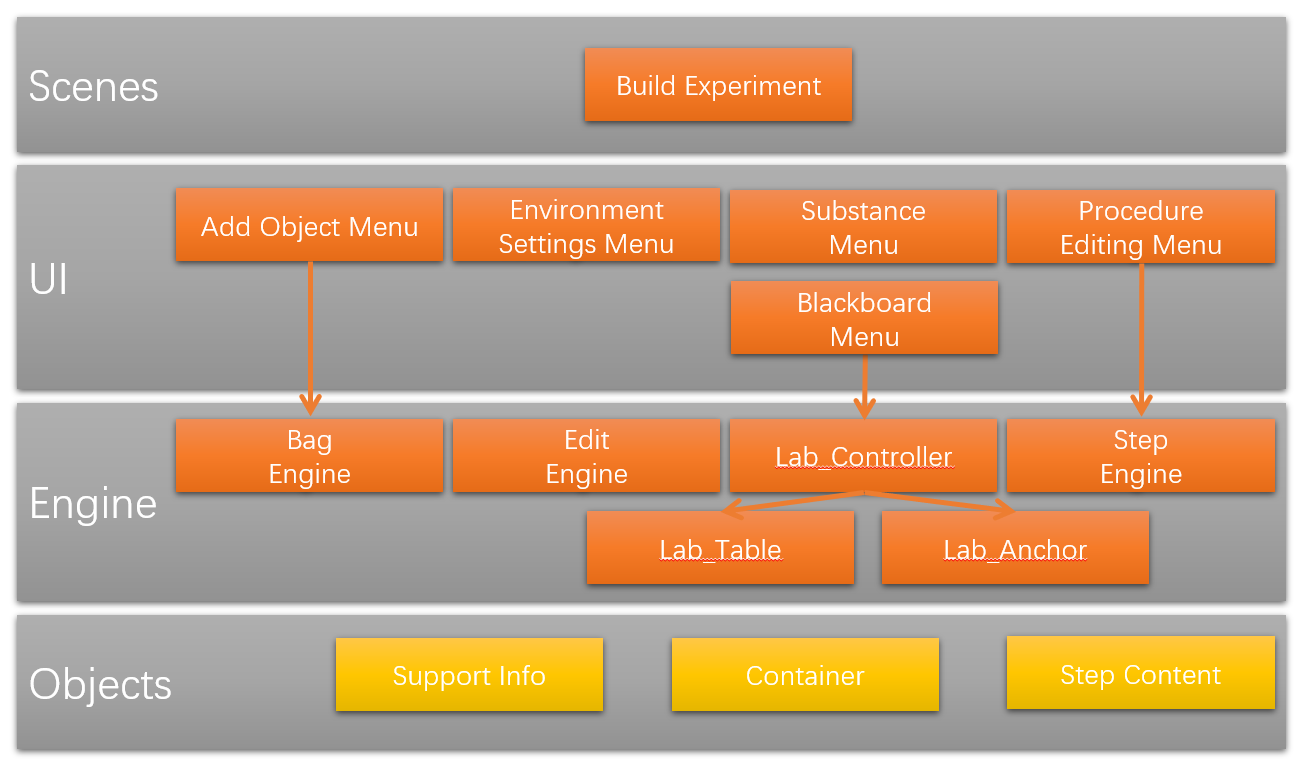
\includegraphics[width=12cm]{figure/buildearc.png}
  \bicaption[编著场景架构设计图]
    {编著场景架构设计图}
    {The Building Experiment Scene Architecture Design}
 \label{fig:gm}
\end{figure}

最上层为用户接口(User Interface,UI),他保存了用户前端的控件。前端控件主要有五个菜单构成。

\begin{itemize}
    \item \textbf{Add Object Menu}
用户可以通过此菜单向场景中添加物体。在菜单中对各类物体进行了分类,对于化学实验来说,包括容器、物质、器具、预置组合四类。
    
    \item \textbf{Environment Settings Menu}
用户可以通过此菜单修改实验场景,例如场景的灯光强度与颜色、室内或是室外环境、相机的高度与角度等。
    
    \item \textbf{Blackboard Menu}
用过可以通过此菜单修改实验中黑板上的实验提示信息的大小、颜色,包括显示实验标题的文字和和显示实验操作和警告的正文两个部分。

    \item \textbf{Substance Menu}
用户可以通过此菜单修改添加的物质的种类和量。

    \item \textbf{Step Menu}
用户可以通过此菜单修改实验的标题、流程、每个流程对应的步骤等内容。由于用户的步骤是多样的,同一个行为可能有多种表达方式,因此系统还提供了事件选项,用与将用户输入的操作以系统中实际实现和判断的操作进行对应。

\end{itemize}
~\\
\indent    	上述的控件需要第二层,引擎进行支撑。由于编著系统很大程度上集中在UI的部分,因此引擎大部分是为UI进行服务的。除了上述的控件之外,还包括应用的其他交互形式,也是由引擎实现的。

\begin{itemize}
    \item \textbf{Bag Engine}
用于控制Add Object Menu。其中包括Menu出现和消失的动画、菜单内部转换逻辑、获取用户希望添加何种物体等功能,并且向更底层的引擎传递用户输入事件。
    
    \item \textbf{Edit Engine}
用于管理编辑场景的所有数据,包括场景中添加物体的位置、种类、容器中的物质或药品的种类与量,黑板文字的位置、颜色、大小,场景中的环境数据等,在编辑完成的时候将所有数据采用固定的格式进行保存,在编辑已有场景的时候从该数据结构中进行读取并且还原。
    
    \item \textbf{Step Engine}
用于控制Step Menu。负责用户创建、编辑每个实验对应的标题、流程、步骤等信息。

    \item \textbf{Lab Controller}
是交互的核心控制引擎,获得鼠标(或手指触摸)事件,运行相应的业务逻辑。判断输入的是点击事件还是长按事件,如果是点击事件则弹出编辑界面,包括提示信息的编辑界面(Blackboard Menu)、物质的编辑界面(Substance Menu)两种。如果是拖动事件,则将被点击的物体或文字进行移动。在编辑已有实验的时候,需要从游戏管理器中读取已创建的物质以及黑板信息数据,并且进行还原。在桌面上拖动时,可以选择固定的锚点上,或是锚点范围外的任意位置。设置锚点的目的是可以使一些仪器保持固定的相对位置和顺序,这些锚点本身是由Lab Anchor进行维护,提供在锚点上添加、替换、删除物体的操作。Lab Anchor由Lab Table进行统一维护,包括在用户在锚点内外删除、移动、添加物体的时候控制所有锚点的行为,例如在用户将物体移入锚点范围的时候,在指定的锚点中空出位置;在用户将物体从锚点拖离的时候,将其他锚点的物体补上空缺等。

    \item \textbf{Button}
对于场景中一直显示的按钮,如展开环境设置菜单的按钮,展开加入物体菜单的按钮等,都在Button中统一实现了点击事件响应函数。他还控制在有面板被展开的时候暂停Lab Controller中物体控制的逻辑,避免用户在使用菜单的时候操作干扰到实验编辑。
\end{itemize}
~\\
\indent    	上述逻辑需要使用一些持久化的对象,用于封装和储存信息,这些对象包括保存用户创建的物质的种类和量的对象Container,保存用户创建的步骤和流程的对象Step Content,保存实验提示信息的颜色和大小信息的text,以及保存系统支持的物质和时间类型的对象Support Info。

此外,由于创新新实验和编辑已有实验共用该场景,因此需要对场景中的编辑数据进行保存,这里使用了类Experiment Setup进行保存。其UML类图\ref{fig:uml}如图所示。


\begin{figure}[!htp]
  \centering
  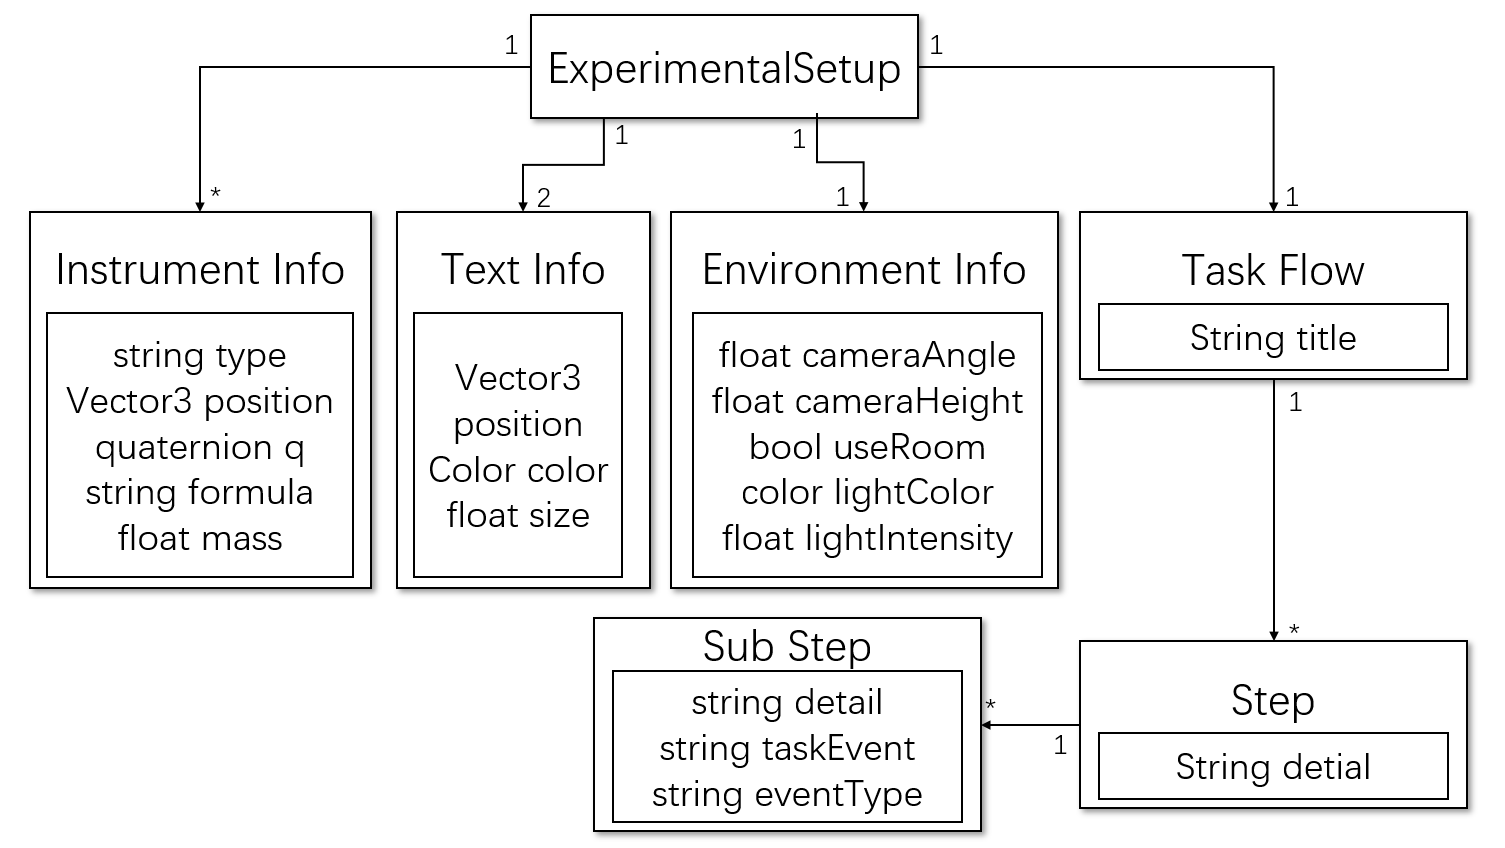
\includegraphics[width=12cm]{figure/setupclass.png}
  \bicaption[编著信息UML类图]
    {编著信息UML类图}
    {The UML's class Diagram of Authored Data}
 \label{fig:uml}
\end{figure}

其中编著信息由四部分组成。每个场景有多个instrument info保存创建的物体的位置、旋转、物体种类、其中含有的物质的名字及其物质的量。每个场景由两个text info,分别用来储存实验提示信息中的标题和正文的位置、大小、颜色信息。每个场景包括一个environment info,用来保存场景中相机、光照的相关属性。每个场景还包括一个task flow,用来保存编辑的实验流程。每个实验流程有多个流程(step),每个流程又有多个步骤(substep),步骤中包含步骤名称、对应的事件等信息。

\subsection{交互场景}
交互场景用于将用户创建的物体根据物体追踪的结果渲染到增强现实场景中。

\begin{figure}[!htp]
  \centering
  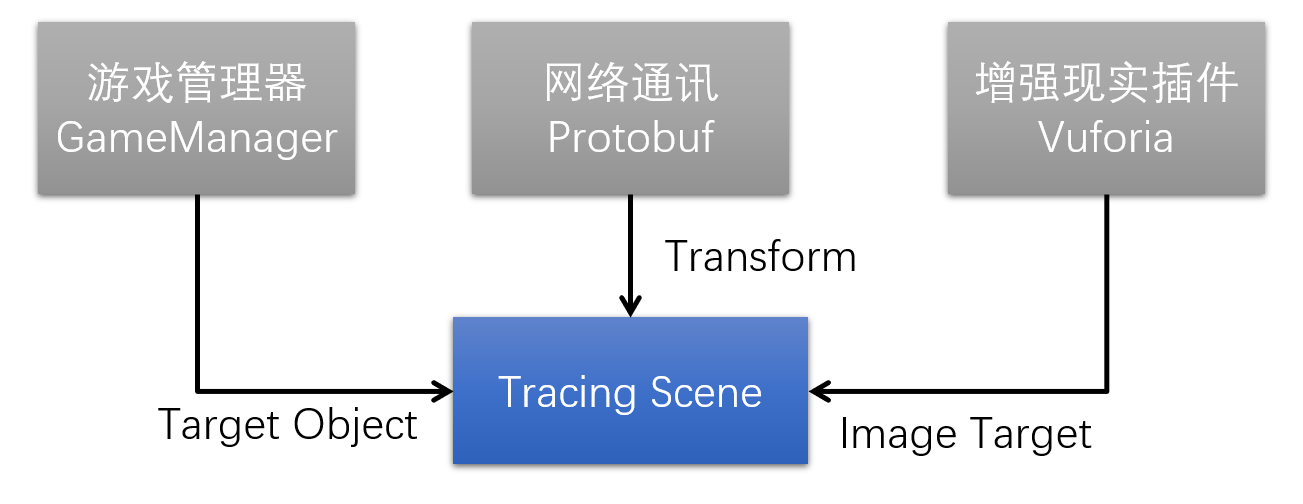
\includegraphics[width=12cm]{figure/tracingScene.png}
  \bicaption[交互场景架构设计图]
    {交互场景架构设计图}
    {The Interaction Scene Architecture Design}
 \label{fig:int}
\end{figure}

场景主要由三个组件构成,首先场景会通过游戏管理器获得要用于显示的被追踪物体的相关数据。然后根据Vuforia识别出场景中的标志物,它用于为Unity确定真实场景的位置和坐标系。之后会打开网络通讯,将追踪结果应用到应被渲染的物体上,就可以实现虚实融合了。


\subsection{其他场景}
除上述场景之外,系统还实现了主页、登录页面、注册页面等场景。它们结构与上述框架类似,而且比较简单。

主页主要负责场景之间的跳转,提供三个按钮,用户用户进入编辑场景、编辑已有场景、进入交互场景。跳转逻辑仍然由游戏控制器负责。

登陆和注册页面前端进行用户输入,然后通过引擎发送网络数据到服务器进行输入检查,如果出现错误则进行错误提示,输入正确的逻辑仍然由游戏控制器负责。

\section{网络通信设计}
\begin{figure}[!htp]
  \centering
  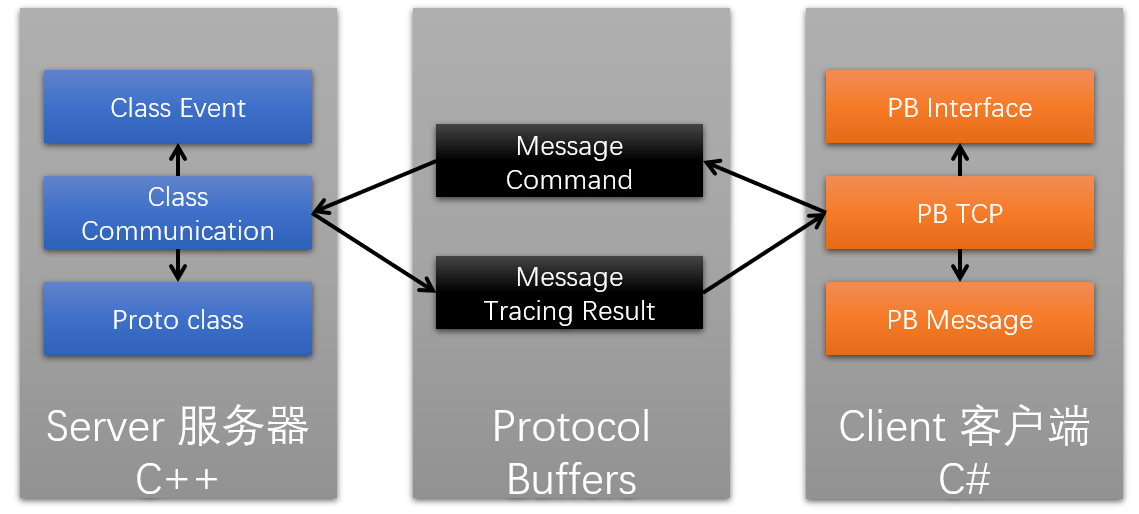
\includegraphics[width=12cm]{figure/netarc.png}
  \bicaption[网络通信架构设计图]
    {网络通信架构设计图}
    {The Network Communication Design Architecture}
 \label{fig:gm}
\end{figure}
应用需要在C++实现的服务器和C\#实现的客户端之间进行通信。通信采用了共同的关键字(Message),在本项目中即command和tracing result。

Command储存的是客户端向服务器发出的指令,包括指令种类,如启动程序录制、启动物体追踪、结束程序等。还包括可选的指令所需要的变量,如追踪物体的种类等。Tracing Result为服务器向客户端返回的追踪结果,是一个由ISRPose的旋转、位移矩阵构成的数组。关键字分别在两端以各自语言中的类表示。

在共同关键字的基础上,两端都实现了各自的socket。服务器在communication类中建立服务,客户端在PB\_TCP中发送请求。服务器获取到客户端请求后通过触发事件运行响应函数。客户端通过PB\_Interface调用相应的函数。

\section{本章小结}
本章介绍了系统的整体架构,包括物体追踪服务器、编著系统客户端、网络通信三部分。并且针对每个部分的架构设计都进行了描述。其中服务器是由多个模块协同完成置顶功能的。而编著系统则按照场景区分编著和增强现实两个主要功能,之后在每个场景中进行了分层的设计。最后网络通讯则通过设定固定的关键字,然后通过两个面向对象的程序中的特定模块进行通信。
